\documentclass[11pt,a4paper]{article}
\usepackage{tikz}
\usetikzlibrary{arrows.meta,positioning}
\usepackage{tabularx}
\usepackage{amsmath,amssymb,amsthm}
\usepackage{geometry}
\geometry{margin=1in}
\usepackage{hyperref}
\usepackage{graphicx}
\usepackage{setspace}
\onehalfspacing

\title{\textbf{Paper C-04: Migration:\\ A Constraint-Driven Flux Dynamics (CDFD) Perspective}}
\author{Steve Bico Mujjabi, MD\\
\small Independent Researcher\\
\small Founder, Vura Labs\\
\small Kampala, Uganda\\
\small ORCID: 0009-0001-0556-5516}
\date{August 2026}

\begin{document}
\maketitle

% BEGIN SHARED-METHODS POINTER
\noindent\textit{Shared Part IV notation and evidence boundaries are defined in \path{PART_IV_METHODS_AND_CLAIM_BOUNDARY.md}. This paper states only its local observables, comparison, and failure conditions.}
% END SHARED-METHODS POINTER


\begin{abstract}
This paper develops a falsifiable CDFD/AFL model of Migration. It maps people, remittances, information, risk, and opportunity gradients to driving flux $\Phi$, borders, cost, housing, jobs, rights, and social acceptance to active constraint $C$, social networks, policy, integration, mobility, and mutual aid to responsiveness $S$, and diaspora ties, path dependence, trauma, law, and settlement history to structural memory $M_s$. The target outcome is movement, welfare, integration, and return or onward migration, tested against censuses, surveys, mobile data, remittances, policy changes, and migration histories. The paper treats universality as a shared model architecture rather than an assertion that unlike systems have the same material mechanism. It states the negative result that would make the mapping unnecessary and places the domain claim inside the cumulative CDFD programme and its reproducible runtime boundary.
\end{abstract}

\section{Introduction}

Physics dictates that fluid will flow from areas of high pressure to areas of low pressure until equilibrium is reached. In the socioeconomic sphere, war, famine, and extreme poverty represent areas of unbearable systemic constraint (high pressure), while prosperous, stable nations represent low-pressure voids. Human migration is the fluid throughput attempting to balance this global thermodynamic equation.

When nations erect physical walls or bureaucratic barriers, they are not halting the pressure gradient; they are merely artificially bottlenecking the flux. Under CDFD, this is a dangerous game of topological brinkmanship.

\section{The Topographic Surface of Migration}
We model international borders utilizing the Adaptive Operating Ratio:
\begin{equation}
    \Psi_s = \left( \frac{\Phi}{C} \right) \cdot S \cdot M_s
\end{equation}

For a national border or immigration system:
\begin{itemize}
    \item \textbf{Flux ($\Phi$)}: The sheer volume of migrants and refugees attempting to cross a geographic threshold.
    \item \textbf{Constraint ($C$)}: The border walls, patrols, visa quotas, and geographic hazards (deserts, oceans) that resist the flow.
    \item \textbf{Responsiveness ($S$)}: The capacity of the host nation's legal and economic systems to process, house, and integrate the incoming population.
    \item \textbf{Memory ($M_s$)}: Nationalistic dogma and entrenched legal bureaucracies. A nation with high institutional memory locks its immigration quotas into rigid, historical configurations, refusing to adapt to real-time global crises.
\end{itemize}

\subsection{Border Crises as Topological Rupture}
When a geopolitical crisis erupts (e.g., a civil war), the push-flux $\Phi$ skyrockets exponentially. If the destination nation has locked its memory ($M_s \to 1.0$) and refuses to increase its processing responsiveness $S$, it must artificially skyrocket its physical constraint $C$ to stop the flow.

Because the pressure gradient is immense, the flux does not disappear; it merely pools at the boundary. The border region enters a state of catastrophic over-flux ($\Psi_s \gg 1$). Refugee camps swell, humanitarian crises erupt, and the physical constraints (walls and patrols) are violently overwhelmed by the sheer thermodynamic weight of the human fluid.

A border system that lacks lawful, humane response capacity may experience abrupt route changes or institutional stress under sustained survival-driven movement; the threshold and outcome are empirical questions.



\section{Measurement Layer}

% BEGIN PART IV MAJOR CROSS-DOMAIN UPGRADE
\section{Cross-Domain Model Upgrade: Mechanism, Scale, and Tests}

\subsection{Observable Translation}

The paper-specific translation begins with an observable chain rather than a
verbal analogy. For Migration, the proposed drive is people, remittances, information, risk, and opportunity gradients.
The active limitation is borders, cost, housing, jobs, rights, and social acceptance. Responsiveness is carried by
social networks, policy, integration, mobility, and mutual aid, while retained state is represented by
diaspora ties, path dependence, trauma, law, and settlement history. The outcome to explain is movement, welfare, integration, and return or onward migration.

\begin{table}[htbp]
\centering
\small
\caption{Operational CDFD/AFL map for Paper C-04.}
\begin{tabularx}{\textwidth}{|l|X|X|}
\hline
\textbf{Term} & \textbf{Paper-specific observable meaning} & \textbf{Measurement question} \\
\hline
$\Phi$ & people, remittances, information, risk, and opportunity gradients & What rate, load, gradient, or demand enters the focal system? \\
\hline
$C$ & borders, cost, housing, jobs, rights, and social acceptance & Which measured bottleneck limits transfer, function, or recovery? \\
\hline
$S$ & social networks, policy, integration, mobility, and mutual aid & Which process changes effective capacity or reroutes the load? \\
\hline
$M_s$ & diaspora ties, path dependence, trauma, law, and settlement history & Which retained state makes equal present loads produce different futures? \\
\hline
$Y$ & movement, welfare, integration, and return or onward migration & Which outcome is predicted out of sample, with uncertainty? \\
\hline
\end{tabularx}
\end{table}

\begin{figure}[htbp]
\centering
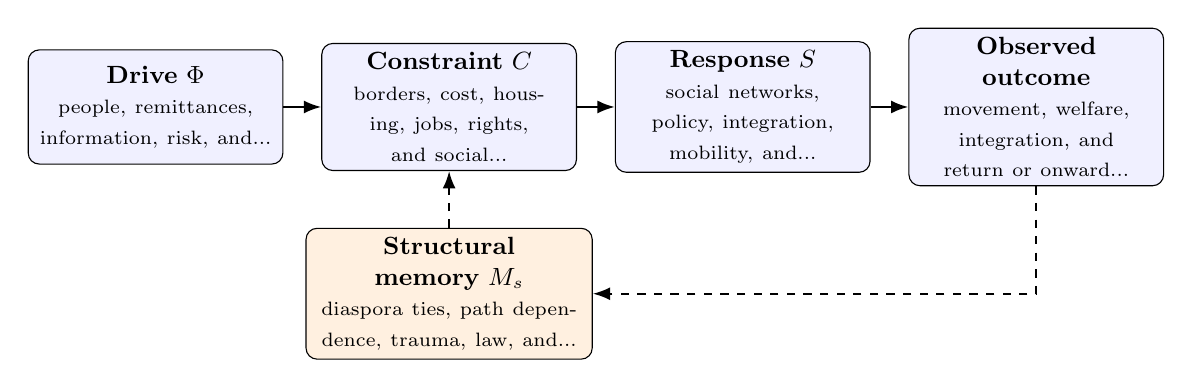
\begin{tikzpicture}[
    node distance=0.48cm,
    every node/.style={font=\small},
    box/.style={draw, rounded corners, align=center, minimum height=1.45cm, text width=3.0cm, fill=blue!6},
    memory/.style={draw, rounded corners, align=center, minimum height=1.25cm, text width=3.4cm, fill=orange!12},
    flow/.style={-{Latex[length=2.2mm]}, thick},
    feedback/.style={-{Latex[length=2.2mm]}, thick, dashed}
]
\node[box] (drive) {\textbf{Drive $\Phi$}\\\scriptsize people, remittances, information, risk, and...};
\node[box, right=of drive] (constraint) {\textbf{Constraint $C$}\\\scriptsize borders, cost, housing, jobs, rights, and social...};
\node[box, right=of constraint] (response) {\textbf{Response $S$}\\\scriptsize social networks, policy, integration, mobility, and...};
\node[box, right=of response] (outcome) {\textbf{Observed outcome}\\\scriptsize movement, welfare, integration, and return or onward...};
\node[memory, below=0.72cm of constraint] (memory) {\textbf{Structural memory $M_s$}\\\scriptsize diaspora ties, path dependence, trauma, law, and...};
\draw[flow] (drive) -- (constraint);
\draw[flow] (constraint) -- (response);
\draw[flow] (response) -- (outcome);
\draw[feedback] (outcome.south) |- (memory.east);
\draw[feedback] (memory.north) -- (constraint.south);
\end{tikzpicture}
\caption{Paper C-04 observable CDFD/AFL architecture for Migration. Solid arrows give the proposed forward chain; dashed arrows make history-dependent feedback explicit.}
\label{fig:c04-architecture}
\end{figure}

\subsection{Paper-Specific Causal Hypothesis}

For this paper, the hypothesized causal sequence is specific. A change in
people, remittances, information, risk, and opportunity gradients arrives faster than social networks, policy, integration, mobility, and mutual aid can compensate.
This raises or redistributes borders, cost, housing, jobs, rights, and social acceptance. If the load persists,
the retained state encoded by diaspora ties, path dependence, trauma, law, and settlement history changes the next response, so a later event of equal
magnitude can produce a different trajectory in movement, welfare, integration, and return or onward migration. The
scientific task is to estimate that sequence against the best ordinary model of
the domain, not merely to redescribe the outcome after it occurs.

\subsection{Cross-Scale Translation Without Mechanistic Erasure}

For the socioeconomic systems family, the cross-domain translation compares human and institutional throughput, unequal access to capacity, adaptive coordination, and historical path dependence. The variables are not morally neutral: aggregation can hide who receives flow, who bears constraint, and whose prior losses become persistent memory. \cite{BarabasiAlbert1999,WattsStrogatz1998,Holling1973,Shannon1948}
The required scale declaration for this paper is days to generations; households to transnational networks. At short
scales, the key question is whether the incoming drive is transmitted,
buffered, or diverted. At intermediate scales, response changes effective
capacity and network exposure. At long scales, retained structure can alter the
state space itself. A result is genuinely cross-scale only when the aggregation
rule is stated and the same conclusion is not an artifact of averaging.

\subsection{Evidence Ladder and Discriminating Tests}

\begin{table}[htbp]
\centering
\small
\caption{Evidence ladder for Paper C-04. Each rung can fail independently.}
\begin{tabularx}{\textwidth}{|p{0.17\textwidth}|X|X|}
\hline
\textbf{Test} & \textbf{Design} & \textbf{Discriminating result} \\
\hline
Proxy audit & Measure censuses, surveys, mobile data, remittances, policy changes, and migration histories and preregister how each record maps to $\Phi$, $C$, $S$, $M_s$, and $Y$. & The mapping fails if proxies are non-identifiable, circular, or change meaning across cases. \\
\hline
Load ramp & Apply or observe a conflict, climate, or labor-market shock across different corridors while estimating the dominant constraint and response time. & A threshold claim requires a reproducible nonlinear change and uncertainty bounds, not a visually chosen breakpoint. \\
\hline
Recovery and memory & Match present load across units with different histories, then compare recovery paths. & The memory claim requires history-dependent divergence after current conditions are controlled. \\
\hline
Model comparison & Compare the baseline domain model with and without the CDFD/AFL state variables using held-out data. & The paper's stated falsifier is: the framework cannot improve explanation after established migration variables are included. \\
\hline
\end{tabularx}
\end{table}

\subsection{Research Programme and Boundary Conditions}

The immediate research programme has four steps. First, construct a documented
dataset from censuses, surveys, mobile data, remittances, policy changes, and migration histories and retain raw units before normalization.
Second, fit a baseline domain model and report its calibration and out-of-sample
error. Third, add the smallest identifiable CDFD/AFL state extension and test
whether it improves prediction of movement, welfare, integration, and return or onward migration. Fourth, repeat the
analysis across the declared scale range and publish negative cases as part of
the cross-domain translation audit.

% END PART IV MAJOR CROSS-DOMAIN UPGRADE

\section{Conclusion}
Migration is shaped by safety, opportunity, rights, policy, cost, social networks, and individual agency. CDFD offers a candidate model of how corridor capacity and institutional response affect movement and welfare; it does not reduce people to fluid or make a policy outcome thermodynamically inevitable.
\section*{Conflict of Interest} The author declares no conflict of interest.
\section*{Data Availability}
Part-specific runtime diagnostics are under each Part's \path{outputs/} directory.

Release-wide code: \path{Part_E_Synthesis/supplementary/}.

Generated summaries: \path{Part_E_Synthesis/outputs/}.

Figures: \path{Part_E_Synthesis/figures/}.


\section{Reference Layer}
\bibliographystyle{plain}
\bibliography{universal_afl_references}
\end{document}
